\section{Neural Network Modeling}
\label{NN}

As it has been stated in the introduction, the modeling of the CHP plant described in the previous section has been performed by means of  NNs. In particular, we have adopted a divide-and-conquer strategy. That is, we have modeled each main component of the plant separately with an NN, and then, we have linked (connected) all the networks by means of shared or common variables (e.g.; an output variable of a network can be an input variable of one or several other networks). The global model is shown in Table \ref{fignns} where a total of twelve NNs are depicted: four for the engines, four for the engine cooling  circuits, one for the exhaust steam boiler, one for the steam turbine condenser, one for the steam turbine and finally another one for the slurry drying process. 

As neural network model, we have selected the well-known multilayer perceptron (MLP) due to its structural flexibility, good representational capabilities and availability of a large number of training algorithms (for example the Back-Propagation algorithm which is the one used here) [Haja2012]. In fact, MLP is an universal approximator and hence it is capable of approximating any measurable function to any desired degree of accuracy \cite{Hornik-1989}. It is understood, therefore, that MLP is the most common used model in those above-cited works that accomplish the modeling of cogenerations processes by means of NNs. In addition, the MLP has not a very complex structure and hence, it can be  used in a cooperative way with the evolutionary algorithm (EA) as proposed in this paper. As it will be explained in Section 4, the EA needs to evaluate the fitness function hundred of times by using the obtained NN models. A NN with a rather complex structure (e.g. recurrent NNs) would lead to a computation time too high for being used in the continuous on-line process of the plant.

In order to select the structure of the MLP model, some initial tests were made using different number of hidden layers. It was concluded that the accuracy did not show any significant improvement after increasing the number of hidden layers. Therefore, the simplest option was selected: only one hidden layer. Similarly, some initial tests were made with different number of hidden nodes. It was concluded that when the number of neurons increases beyond twice the number of inputs (i.e., a common practical rule), results barely improve. Therefore, the adopted criterion in all the models is, using twice as many hidden nodes as the number of inputs.

In our modeling,  each NN computes a single output, which in some cases becomes the input for another model (see Table \ref{fignns}).  These outputs are respectively: a) the temperature of the water to cool each engine ($T_{Mixt\_EngA}$, \dots, $T_{Mixt\_EngD}$; b) the flow of fuel (i.e. natural gas) required by each engine ($F_{Gas_A} \dots F_{Gas_D}$); c) the pressure of the condenser ($P_{CON}$); d) the steam flow in the boiler ($F_{Steam}$); e) the electric power produced by the turbine ($POW_{ST}$) and f) the flow of slurry processed by the evaporator ($F_{EV}$).

\begin{table}[!t]
\caption{CHP Neural-Networks and their corresponding variables.}
\label{fignns}
  \centering
\begin{tabular}{lll} \toprule
 Neural-Network  & Inputs of the model & Output \\ \midrule
Cooling Engine A & $\bf{T_{H2O\_Ex}}$, $T_{H2O\_TOW}, POW_A $ & $T_{Mixt\_EngA} $ \\
Cooling Engine B & $\bf{T_{H2O\_Ex}}$, $T_{H2O\_TOW}, POW_B $ & $T_{Mixt\_EngB} $ \\
Cooling Engine C & $\bf{T_{H2O\_Ex}}$, $T_{H2O\_TOW}, POW_C $ & $T_{Mixt\_EngC} $ \\
Cooling Engine D& $\bf{T_{H2O\_Ex}}$, $T_{H2O\_TOW}, POW_D $ & $T_{Mixt\_EngD} $ \\

 Engine A& $\bf{T_{B1\_A}, T_{B2\_A}}$, $T_{Amb}, H_{Amb}, LHV $ & $F_{Gas\_A} $ \\
 & $T_{Bank1\_A}, T_{Bank2\_A}, T_{Mixt\_EngA}, POW_A, DIV_A $ &  \\
 
 Engine B& $\bf{T_{B1\_B}, T_{B2\_B}}$, $T_{Amb}, H_{Amb}, LHV $ & $F_{Gas\_B} $ \\
 & $T_{Bank1\_B}, T_{Bank2\_B}, T_{Mixt\_EngB}, POW_B, DIV_B $ &  \\
 
 Engine C& $\bf{T_{B1\_C}, T_{B2\_C}}$, $T_{Amb}, H_{Amb}, LHV $ & $F_{Gas\_C} $ \\
 & $T_{Bank1\_C}, T_{Bank2\_C}, T_{Mixt\_EngC}, POW_C, DIV_C $ &  \\
 
 Engine D& $\bf{T_{B1\_D}, T_{B2\_D}}$, $T_{Amb}, H_{Amb}, LHV $ & $F_{Gas\_D} $ \\
 & $T_{Bank1\_D}, T_{Bank2\_D}, T_{Mixt\_EngD}, POW_D, DIV_D $ &  \\ 
 
Exh. steam boiler & $\bf{P_{StGen}}$, $F_{FlueGas}$ & $F_{Steam} $ \\
Steam turbine & $T_{H2O\_TOW}, T_{ST\_Cond}$ & $P_{Cond} $ \\
Condenser & & \\
Steam turbine & $P_{StGen}, F_{Steam}, P_{Cond}$ & $POW_{ST} $ \\
Slurry process & $\bf{P_{EV}, T_{H2O\_SH}, T_{H2O\_Ex}}$, $F_{Cond} $ & $F_{Ev}$ \\ \midrule


\end{tabular}
\vspace{-0.3cm}

\end{table}

To train and test the NNs, a big and complete data set was collected trough a one-year observation process in the real plant.  213 parameters were identified as being potentially relevant for training and validating the NN models. Their values have been measured and retrieved with a resolution of one minute during the whole period of observation. Firstly, a careful analysis of the data was performed to choose the most relevant variables and also to filter outliers, missing data or un-informative variables. Next, based on previous knowledge of the system physics and also on a trial/error process, we determined the particular input variables involved in each NN. Table \ref{fignns} shows which are the input/output variables for the different NNs. The variables written in bold refer to the decision variables that will be used later in the optimization process. To make the huge data set more tractable, we have selected 10-minute separated values. This action can be realized, because we have observed that the variables change very little in that period, due to the slow dynamics of the plant. We, thus, obtain a total of about \num{40000} samples for each variable. Now, for making the NNs capable of modeling the different dynamics of the process throughout the whole year, we have made the training/testing partition in the following way: data from odd months (i.e., January, March, May, \dots) are used to train the models, and data from even months (i.e., February, April, June, \dots) are used to test the modeling performance of the trained NNs. The whole training/testing process has been carried out by using the Optibat trainer Tool \cite{Optibat}.

%\begin{figure}
%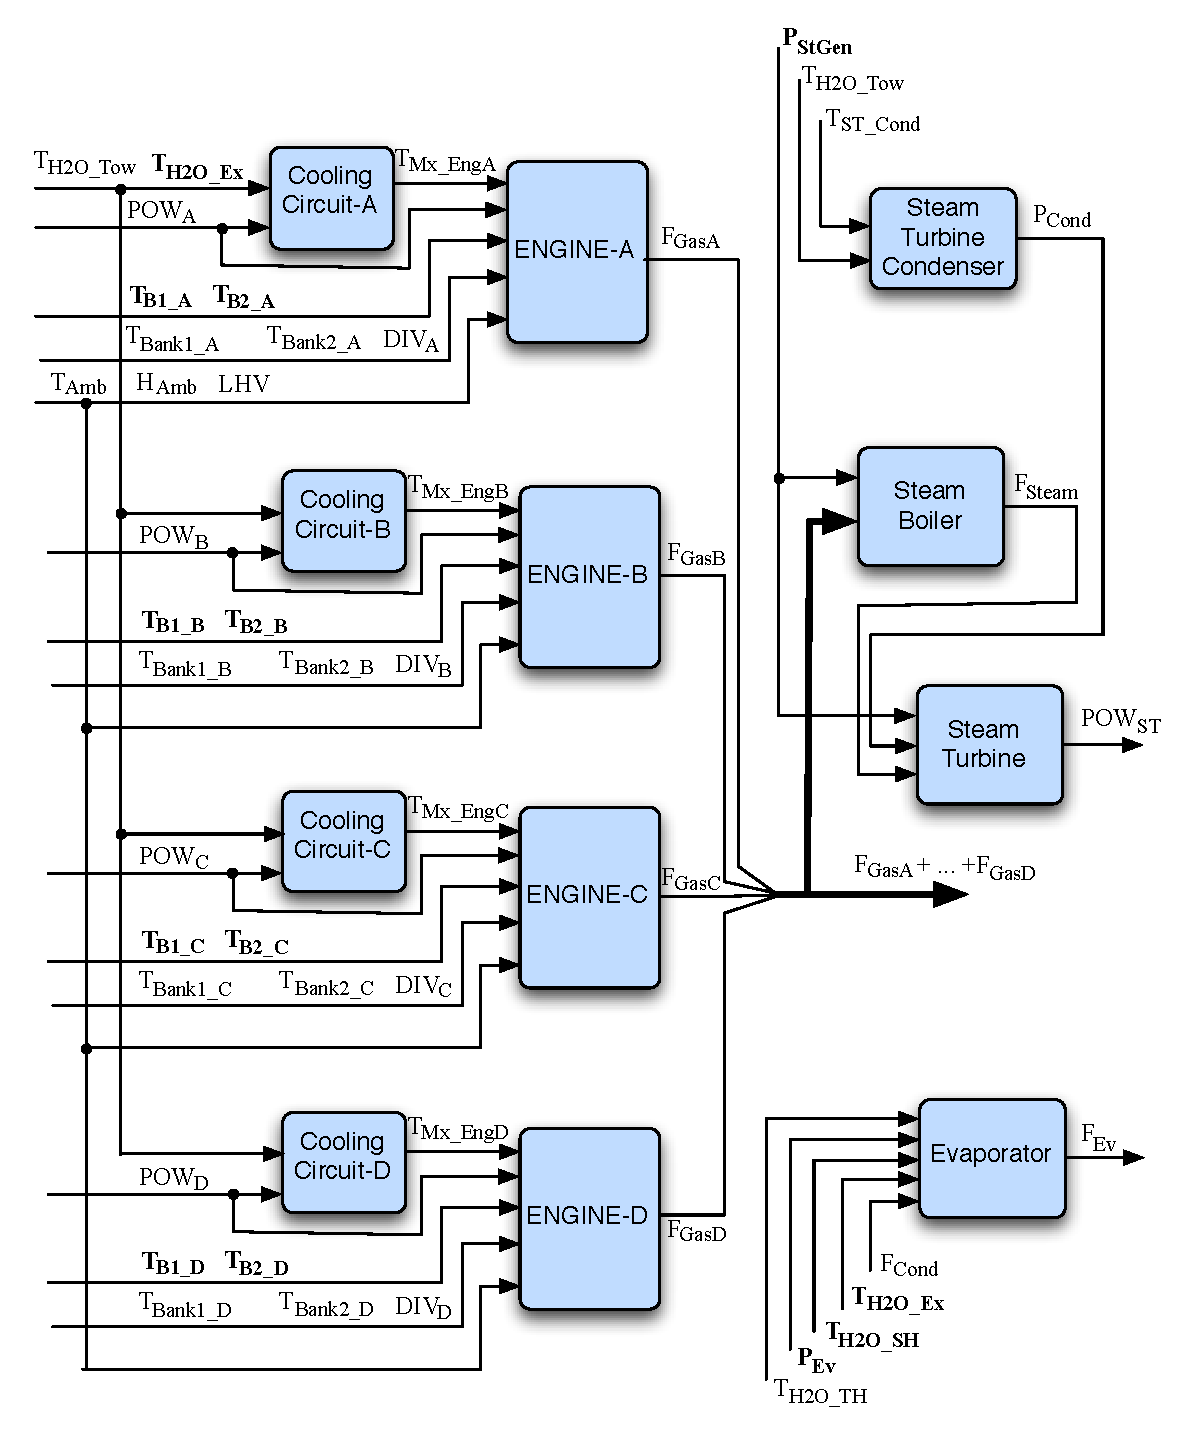
\includegraphics[width=1\textwidth]{NNs.pdf}
%\caption{Modeling of the CHP Plant by means of interconnected NNs. Each block represents an NN.}
%\label{fignns}
%\end{figure}

The results of the modeling are presented in Table \ref{tbl:mse}, where the mean squared error (MSE) between the desired and actual output, for both the training and the testing phase, is shown. We can see that, in all the cases, the obtained  errors are very small. More precisely, most of the models provide a training error less than \SI{1}{\percent}. Even in the testing case, where the NNs deal with unseen data, the error is quite small. Note that the testing error represents the model's behavior better than the training error as it contains unseen data during the training of the models. Hence, the testing error is used to evaluate the  model's  predictive behavior. We can see that for all the models, the difference between the training error and the testing error was always less than \SI{0.3}{\percent}. This means that the models were capable of learning the dynamic of the systems and can make accurate predictions when dealing with unseen data. These results validate the modeling performance of the trained NNs. 



\begin{table}[!t]
\caption{MSE for training and testing samples for each Neural Network.}
\label{tbl:mse}
  \centering
\begin{tabular}{lrrrr} \toprule
 & Structure  & Training Error & Testing Error \\ \midrule
Cooling Engine A & 3/6/1 & \SI{0.21}{\percent} & \SI{0.23}{\percent} \\
Cooling Engine B & 3/6/1  & \SI{0.28}{\percent} & \SI{0.26}{\percent} \\
Cooling Engine C & 3/6/1  & \SI{0.10}{\percent} & \SI{0.13}{\percent} \\
Cooling Engine D & 3/6/1  & \SI{0.49}{\percent} & \SI{0.33}{\percent} \\
 Engine A & 10/20/1  & \SI{0.39}{\percent} & \SI{0.42}{\percent} \\
 Engine B & 10/20/1  & \SI{0.41}{\percent} & \SI{0.41}{\percent} \\
 Engine C & 10/20/1  & \SI{0.38}{\percent} & \SI{0.42}{\percent} \\
 Engine D & 10/20/1  & \SI{0.38}{\percent} & \SI{0.37}{\percent} \\
 Recovery Boiler & 2/4/1  & \SI{0.61}{\percent} & \SI{0.63}{\percent} \\
 Steam Condenser & 2/4/1  & \SI{1.01}{\percent} & \SI{0.96}{\percent} \\
 Steam Turbine & 3/6/1  & \SI{0.67}{\percent} & \SI{0.70}{\percent} \\
 Slurry Process & 5/10/1  & \SI{2.35}{\percent} & \SI{2.52}{\percent} \\
 \bottomrule
\end{tabular}
\vspace{-0.3cm}

\end{table}

For better appreciating the modeling ability of the NNs, we have also plotted the difference between the predicted data and the real data for the testing points (Figures \ref{TcoolA} to \ref{PEvaporator}). Because the four cooling-circuit models and the four engine models have  similar behavior, we have plotted only the output variables of six of the twelve models: $T_{Mixt\_EngA}$, $F_{GasD}$, $P_{Cond}$, $F_{Steam}$, $POW_{ST}$ and $F_{Ev}$.  We can observe in these figures how, although there exists some peaks (which in somes cases they are due to outliers or unusual values) the values of these differences are in general small. In particular the mean value of these differences is below the 0.65\% in all the cases, being the model for the $T_{Mixt\_EngA}$ the best case (0.08\%) and the model for the $F_{Ev}$ the worst case (0.65\%). Thus, it is confirmed that the NNs are able to learn rather well the dynamics of the plant.


\begin{figure}
\centering
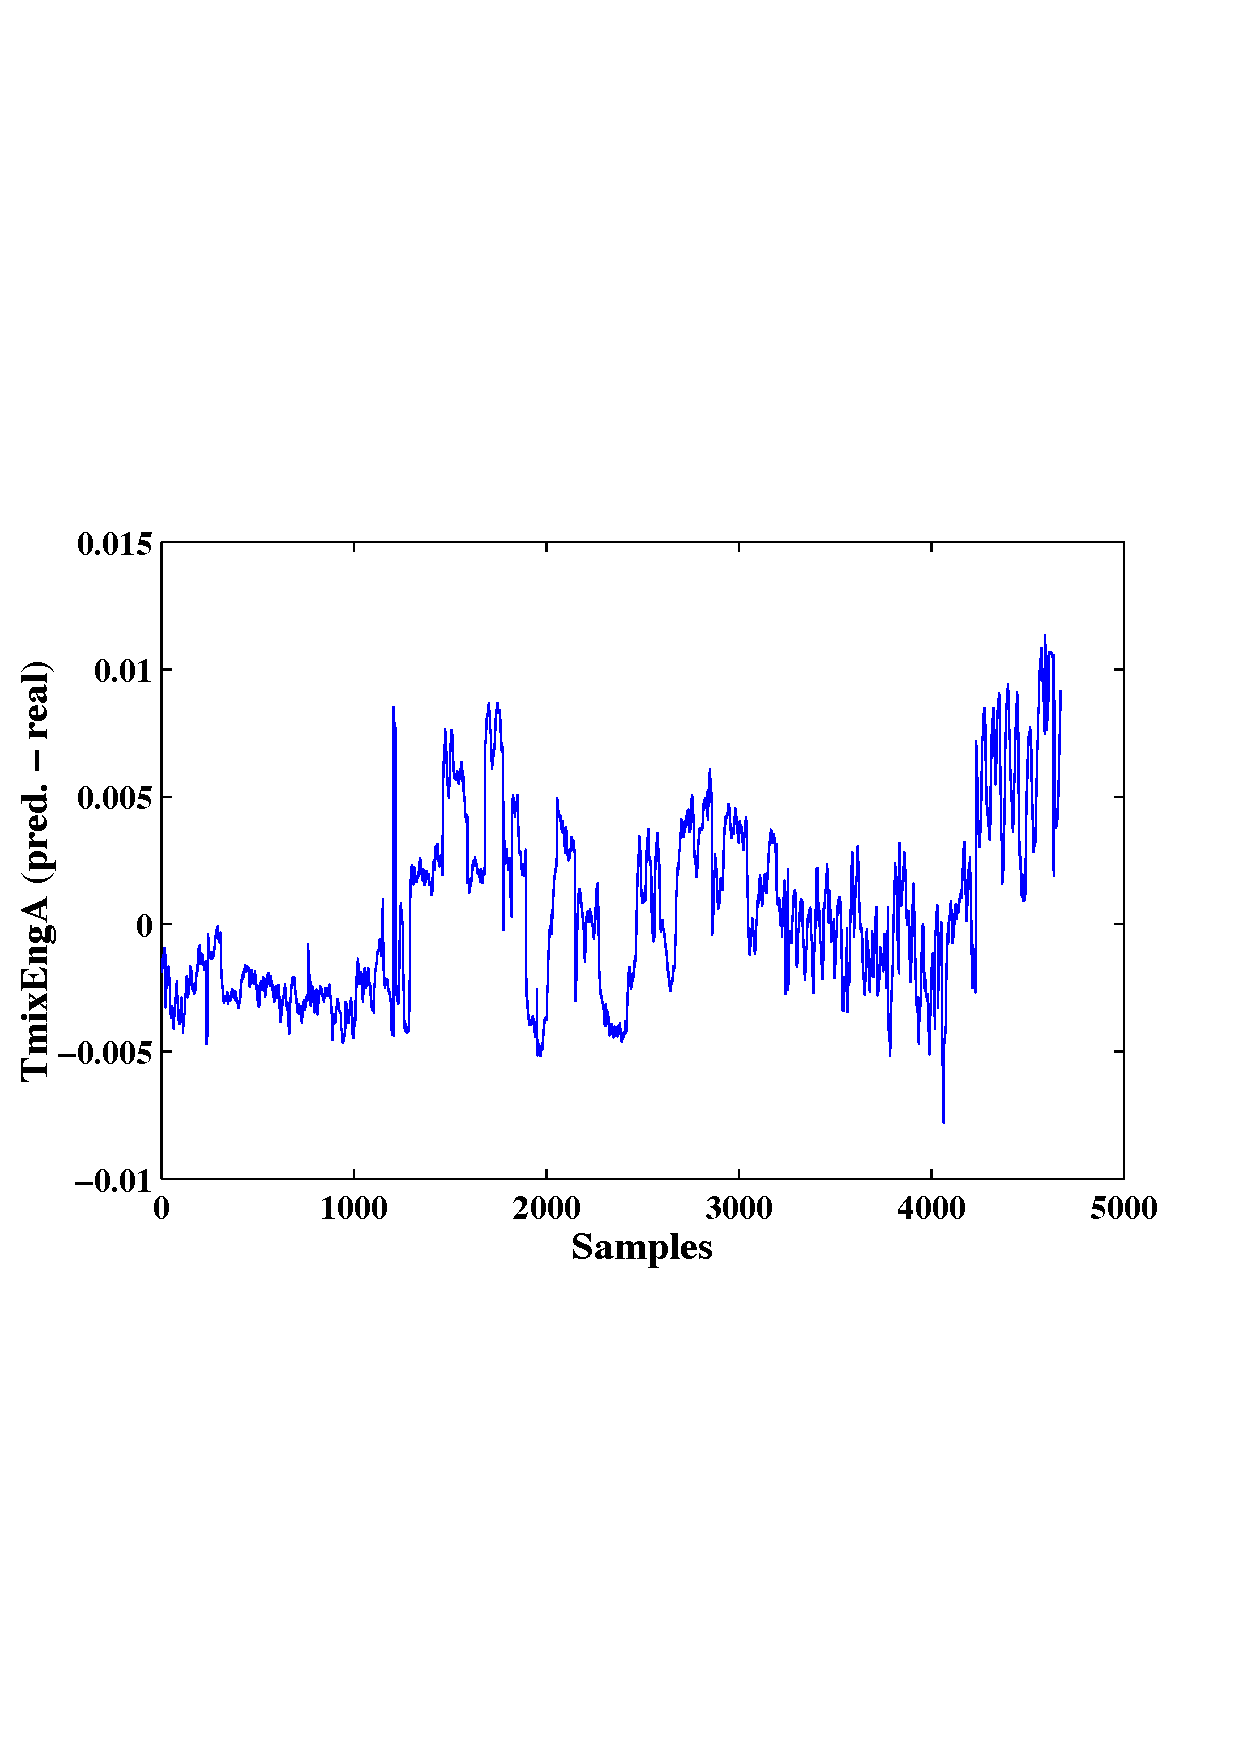
\includegraphics[width=1\textwidth]{figures/TmixEngAdiff.pdf}
\caption{Difference between real data and NN predicted data for the cooling circuit temperature of Engine A ($T_{Mixt\_EngA}$).}
\label{TcoolA}
\end{figure}

\begin{figure}
\centering
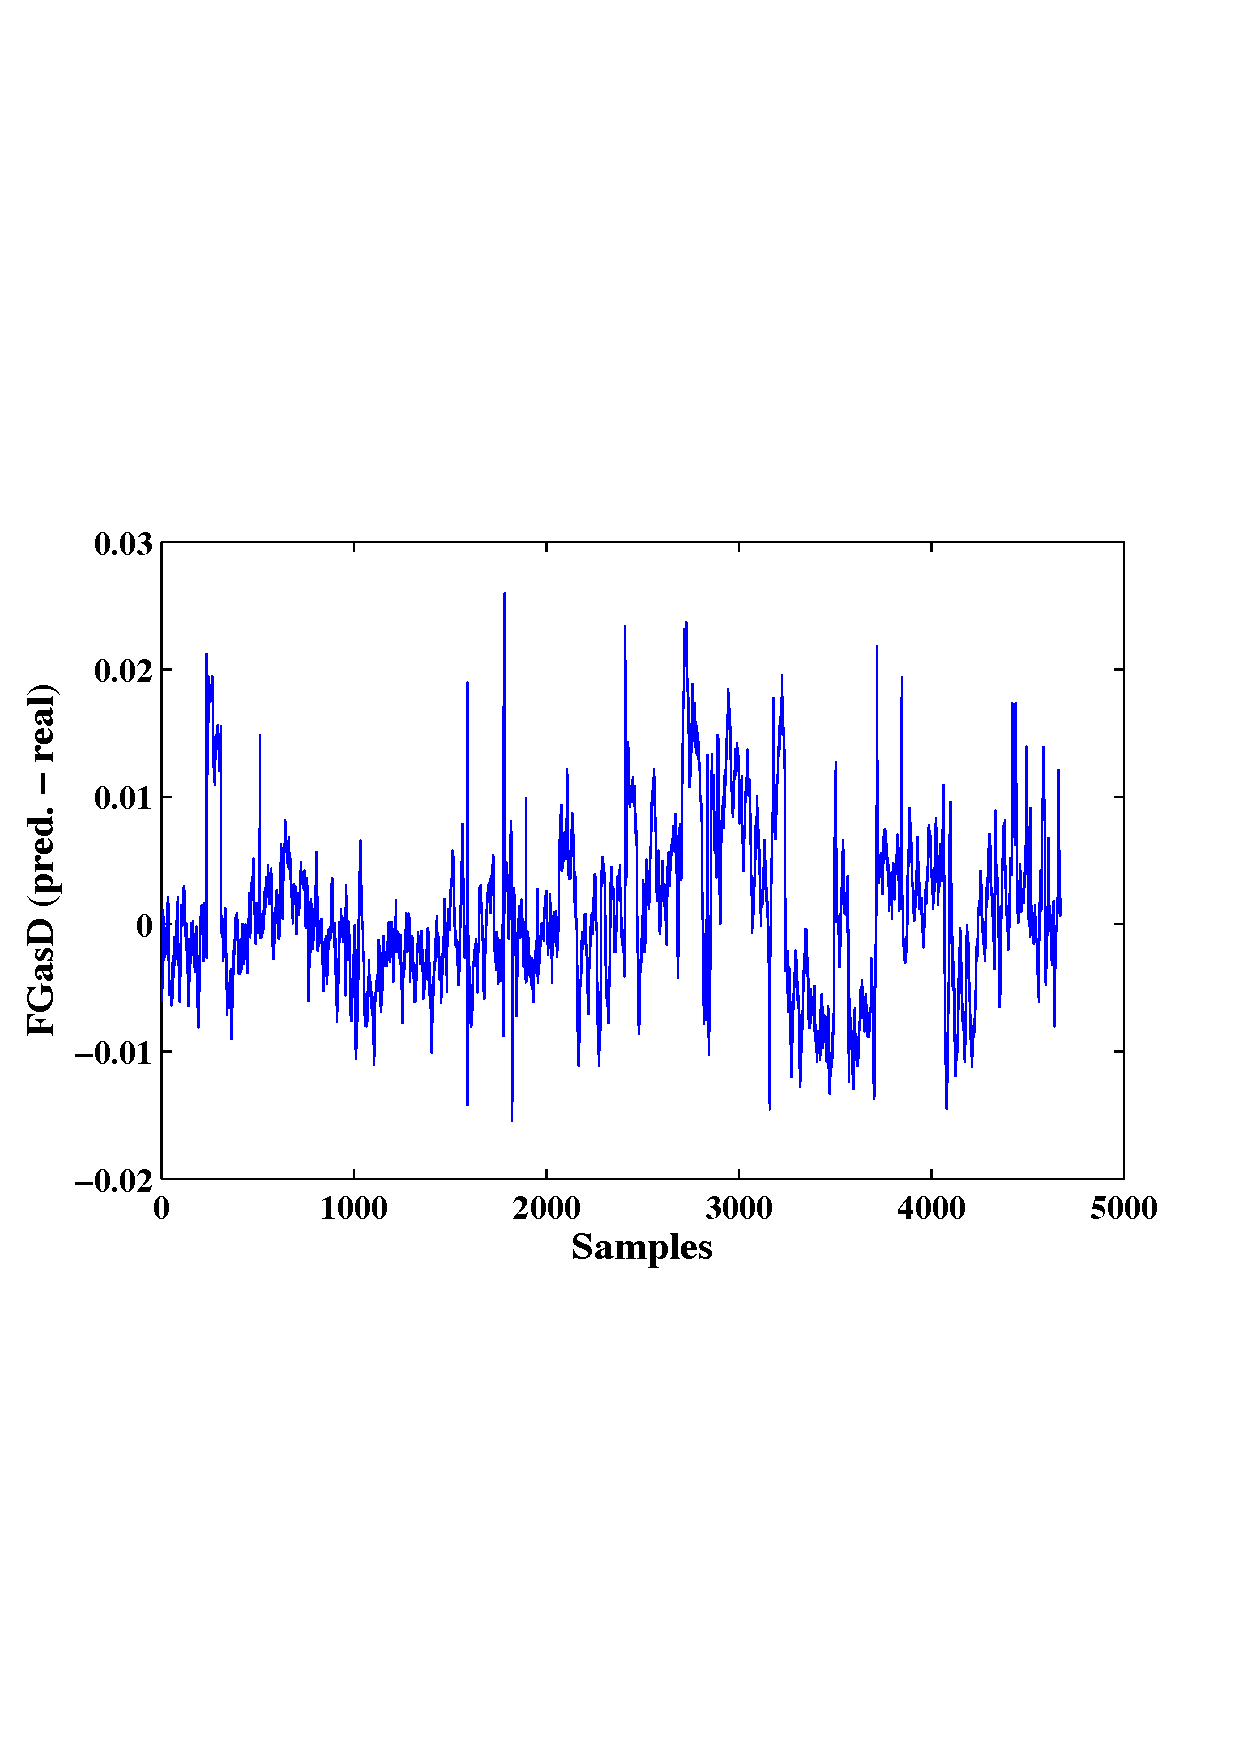
\includegraphics[width=1\textwidth]{figures/FGASDdiff.pdf}
\caption{Difference between real data and NN predicted data for the natural gas flow  of Engine A ($F_{GasA}$).}
\label{FengineA}
\end{figure}

\begin{figure}
\centering
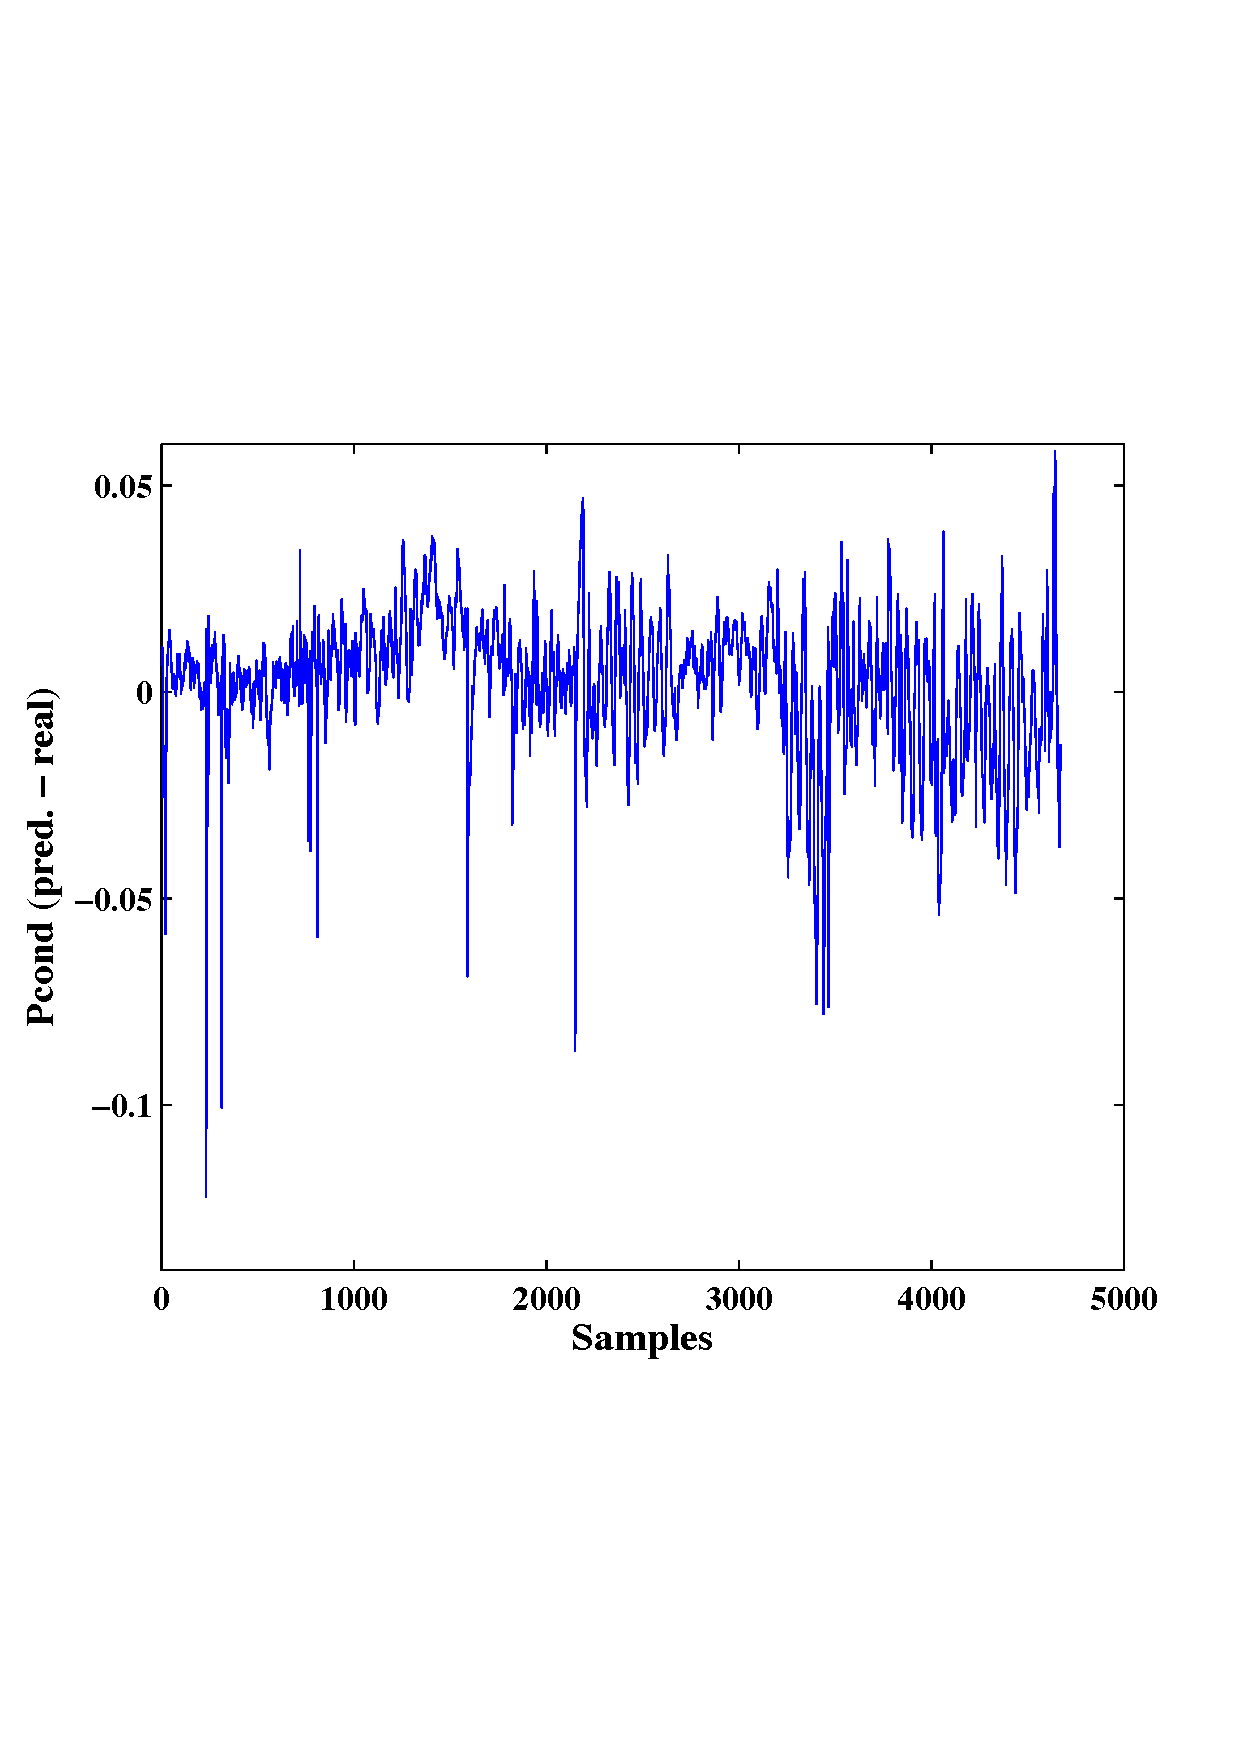
\includegraphics[width=1\textwidth]{figures/Pconddiff.pdf}
\caption{Difference between real data and NN predicted data for the steam pressure of the condenser  ($P_{Cond}$).}
\label{Pcond}
\end{figure}

\begin{figure}
\centering
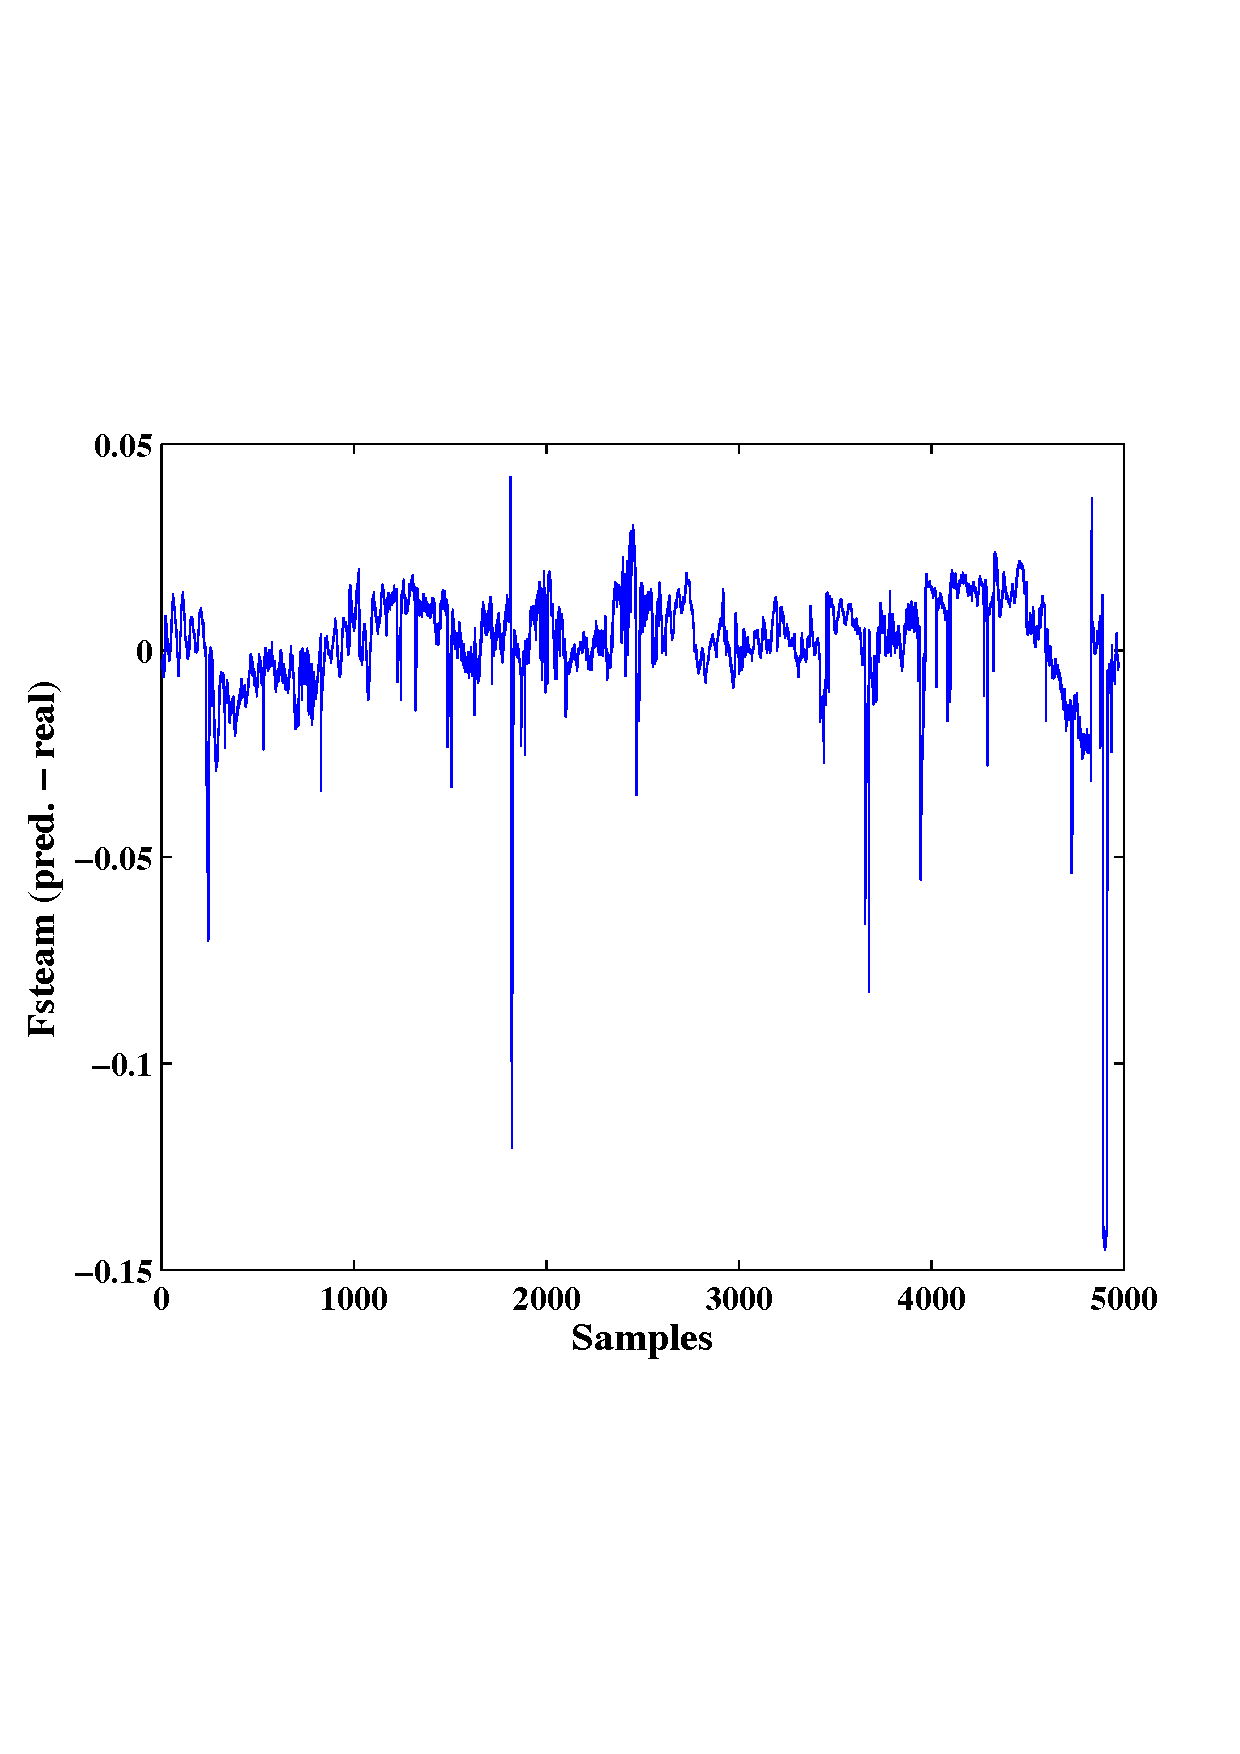
\includegraphics[width=1\textwidth]{figures/Fsteamdiff.pdf}
\caption{Difference between real data and NN predicted data for the steam flow in the boiler ($F_{Steam}$).}
\label{Fboiler}
\end{figure}

\begin{figure}
\centering
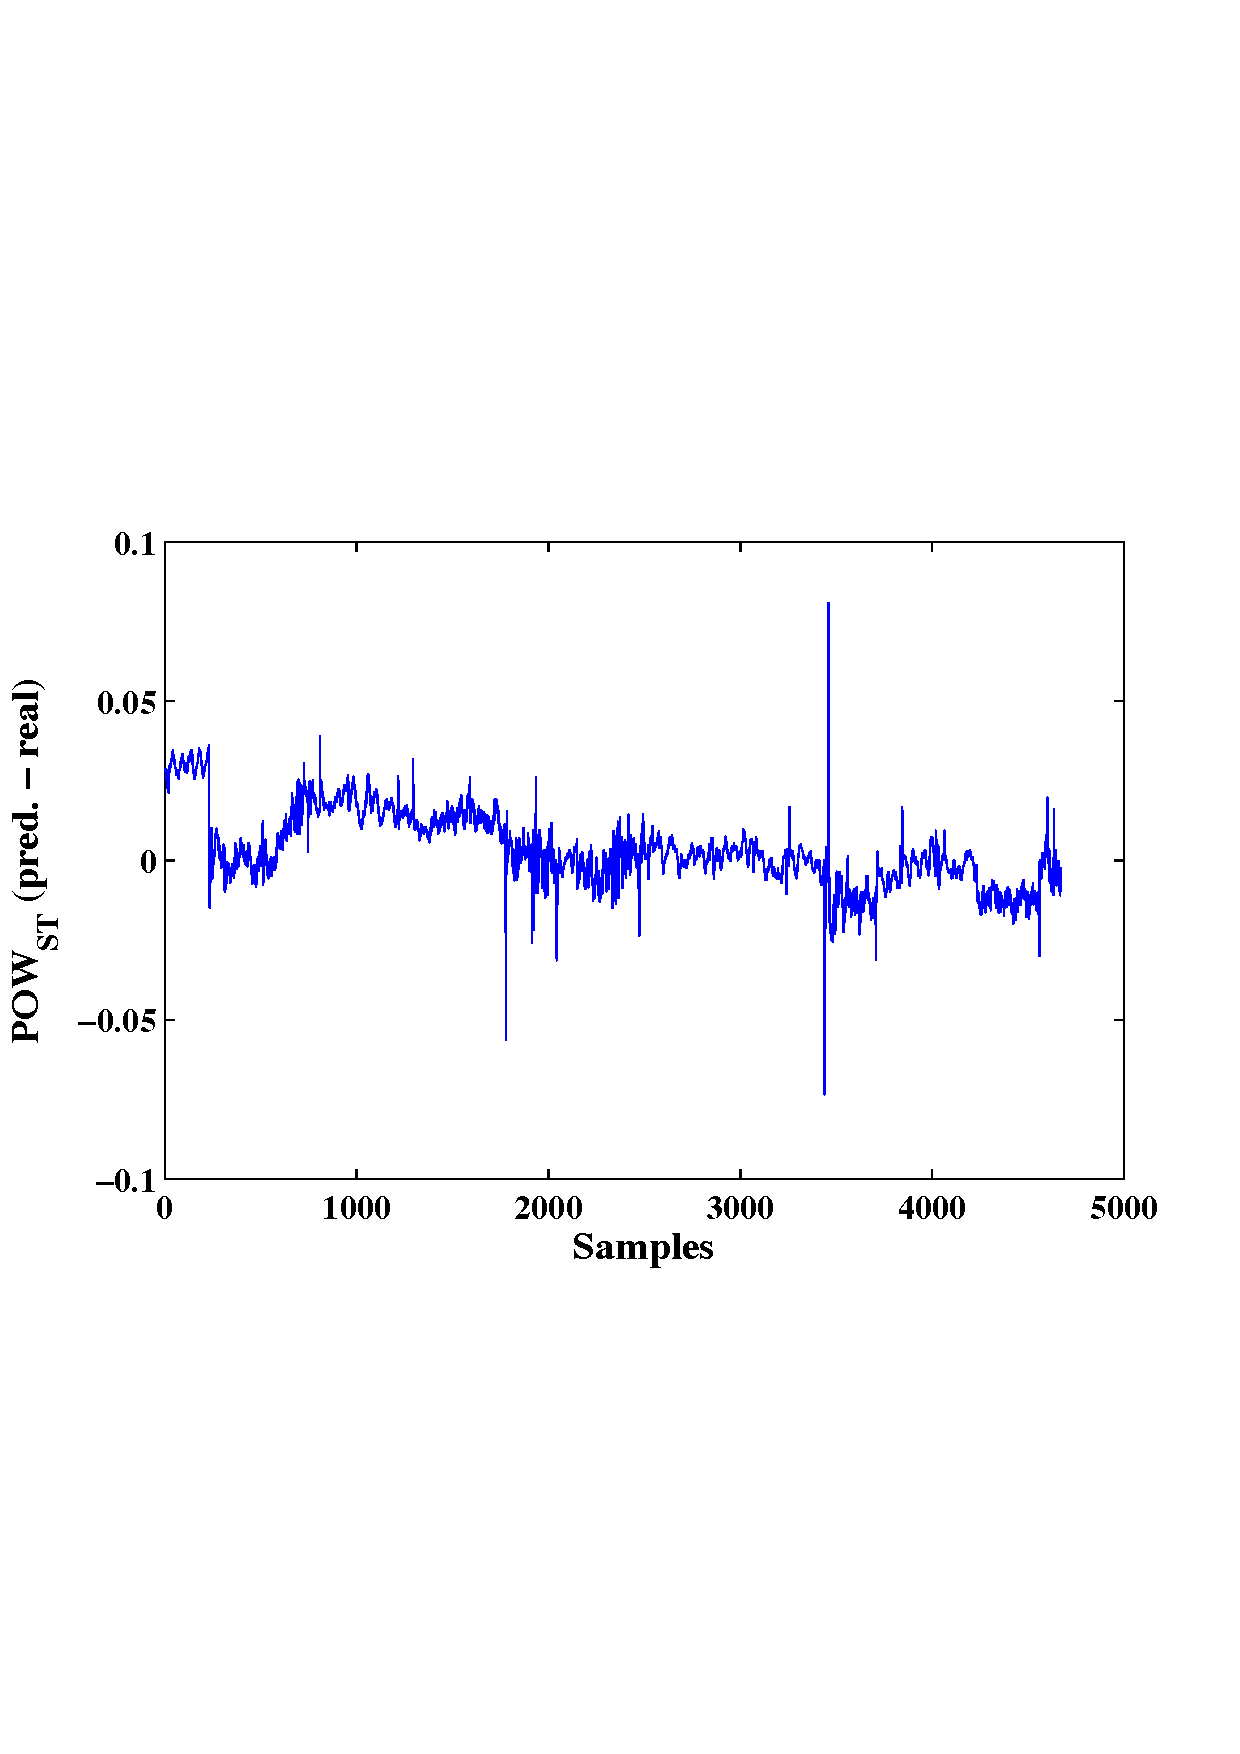
\includegraphics[width=1\textwidth]{figures/POWdiff.pdf}
\caption{Difference between real data and NN predicted data for the Power generated in the Turbine ($POW_{ST}$).}
\label{Pturbine}
\end{figure}

\begin{figure}
\centering
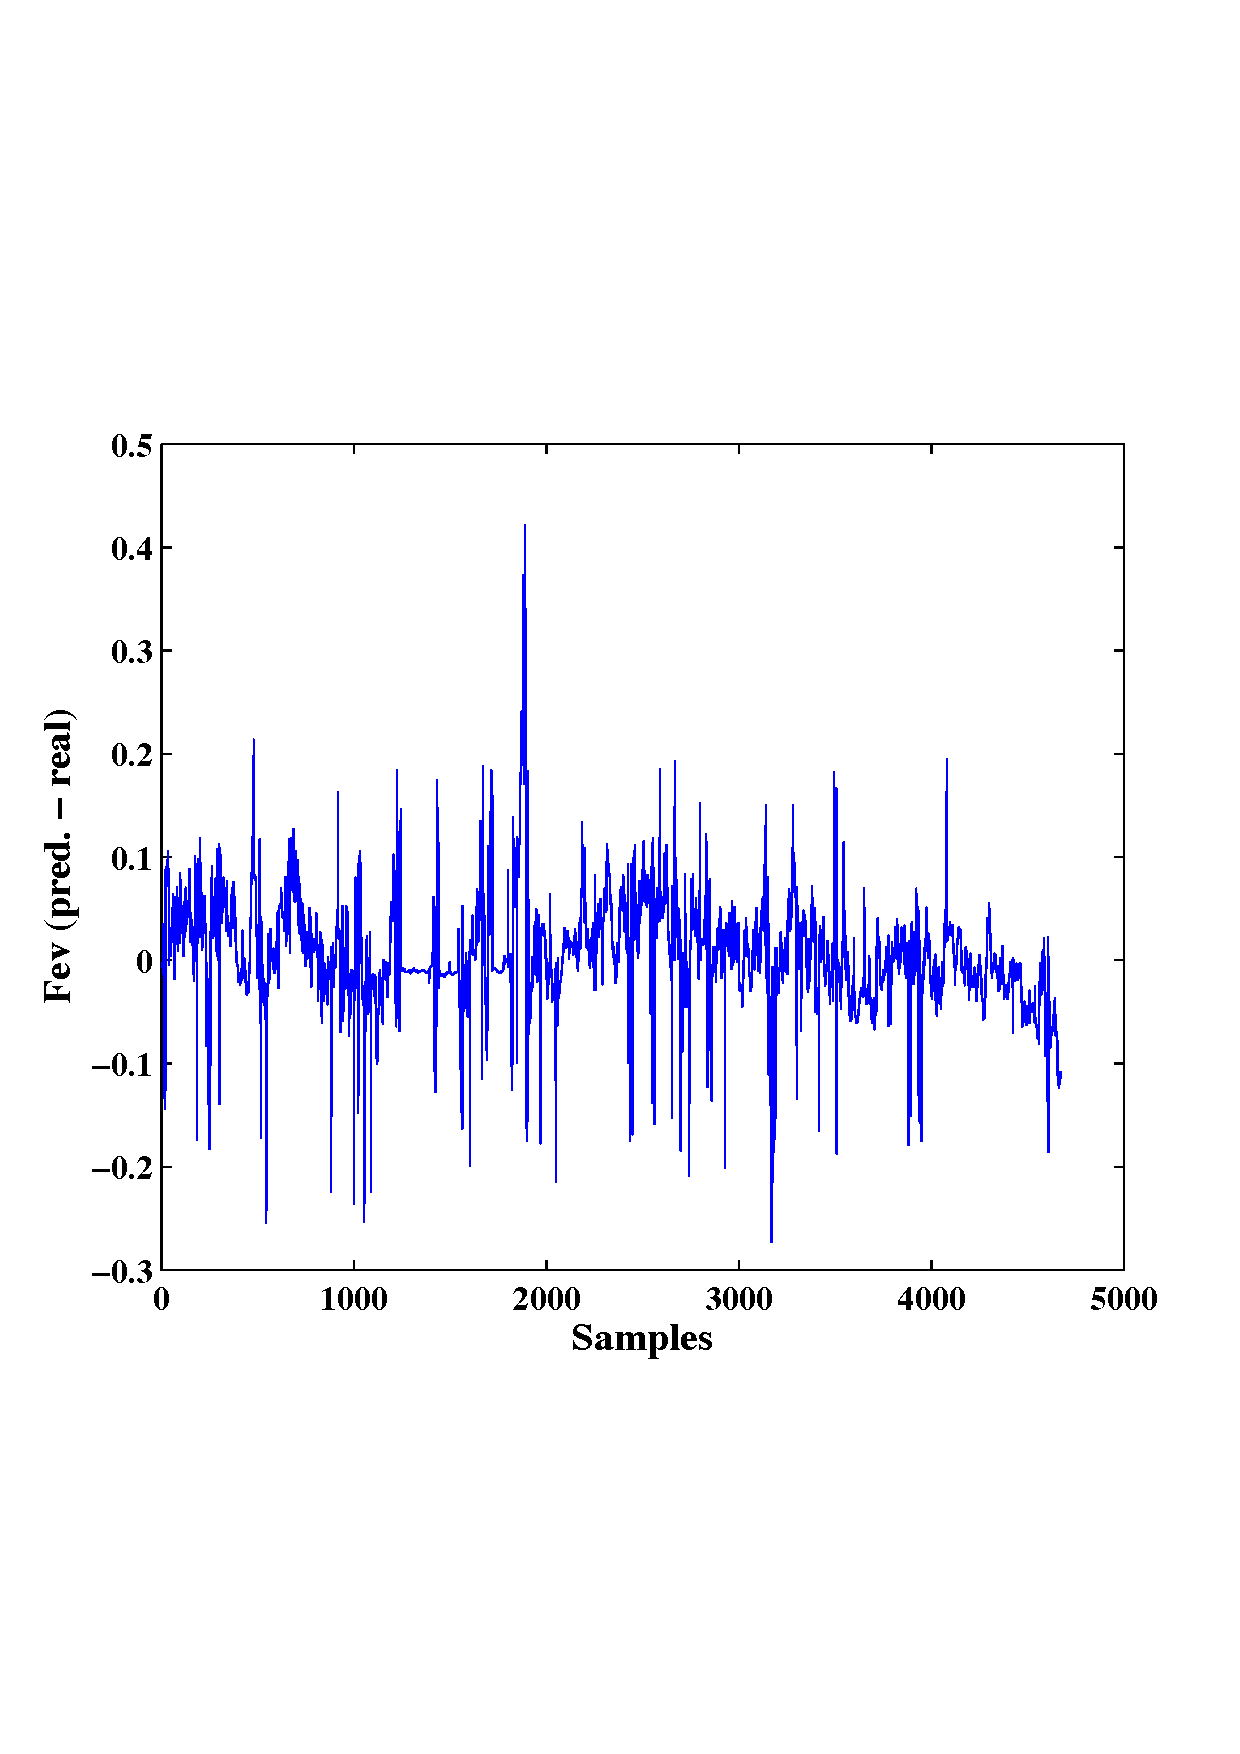
\includegraphics[width=1\textwidth]{figures/Fevdiff.pdf}
\caption{Difference between real data and NN predicted data for the Slurry drying process ($F_{Ev}$).}
\label{PEvaporator}
\end{figure}
